\section{Le matériel expérimental}

\subsection{Scintillateurs}

\subsection{Photo-multiplicateurs}

\begin{figure}
    \centering
	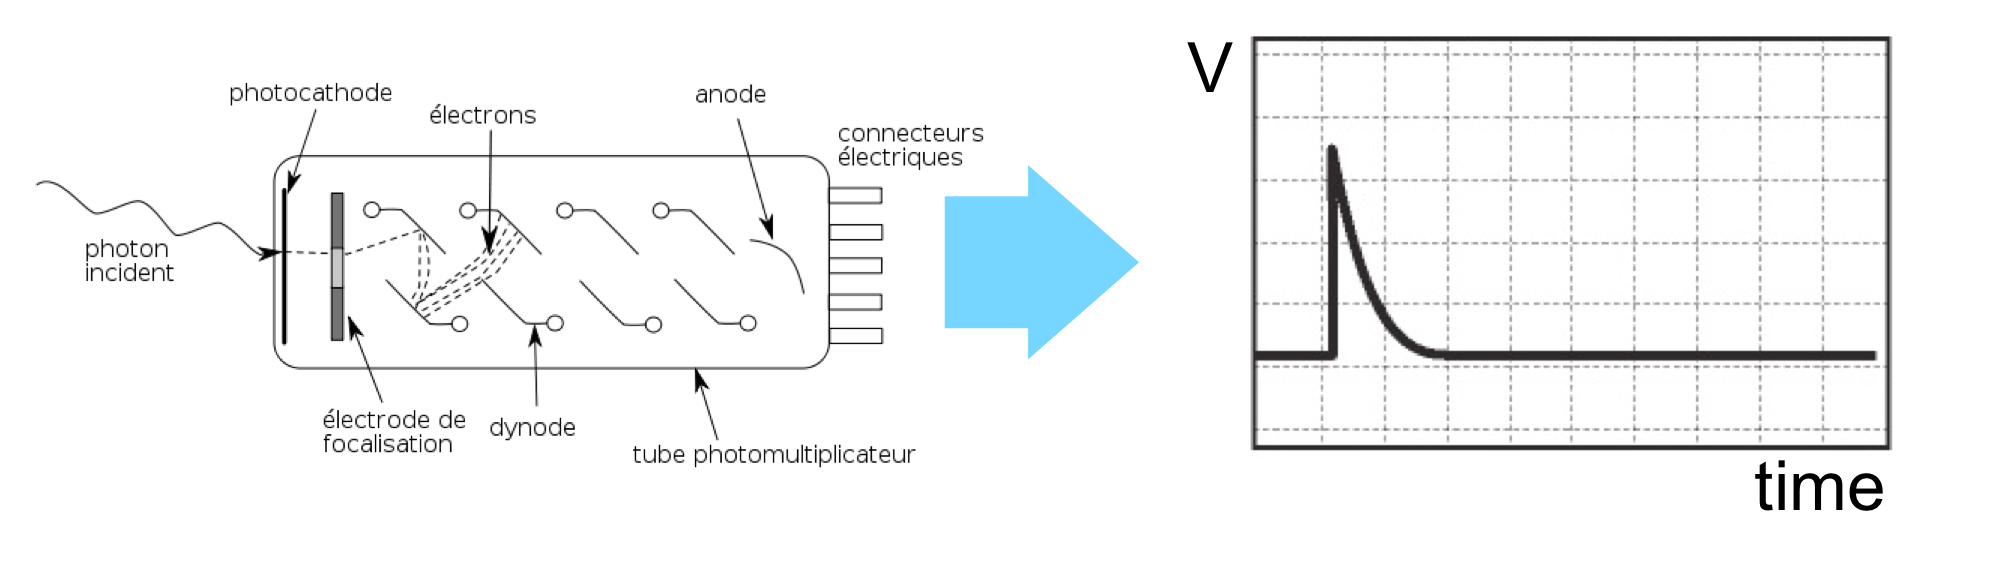
\includegraphics[width=\textwidth]{figures/PMT_readout.png}
    \caption{Schema du fonctionnement d'un photo-multiplicateur(PMT).}
    \label{fig:PMT_readout} 
\end{figure}

Nous allons à présent étudier les différentes composantes d'un spectre en charge typique de la réponse d'un photo-multiplicateur.\\

\begin{figure}[!h]
    \center{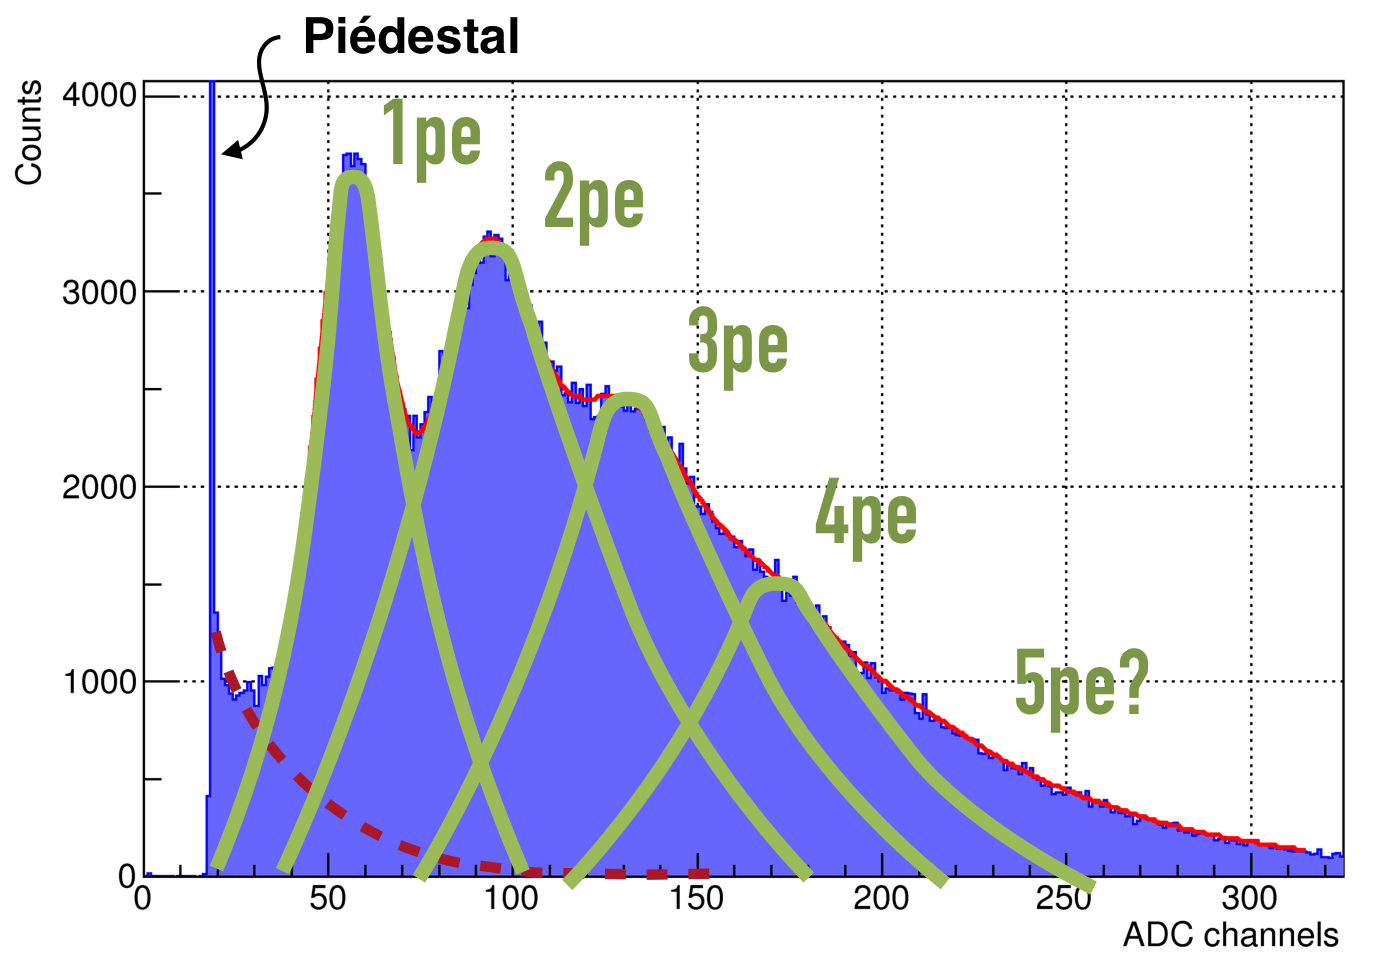
\includegraphics[width=0.7\textwidth]
    {figures/SpectreEnCharge.png}}
    \caption{\label{fig:spectre} Spectre en charge d'un photo-multiplicateur.}
\end{figure}

\textbf{Piédestal :} Il s'agit d'évènements sans charge qui prennent la forme d'un pic en zéro. Afin de se débarrasser de cet effet, il vous faudra régler au mieux votre seuil.\\

\textbf{Dark current :} Il s'agit de bruit associé au PM, il survient lorsqu'un électron est arraché à une dynode sans qu'un photon incident n'arrive à la photo-cathode. Il nous donne une exponentielle décroissante. Cet effet est exacerbé lorsque la tension aux bornes du photo-multiplicateur est élevée. \\

\textbf{Pic des photo-électrons :} Ce sont le réponse en charge du PM pour différent nombre de photo-électrons.\\

Le largeur de la gaussienne du premier photo-électron (1pe) va nous donner la résolution en charge du PM. La relation entre la hauteur des gaussiennes nous est donné par la distribution de Poisson.

\subsection{Aquisition de donn{\'e}es}

\begin{figure}
    \centering
    \begin{subfigure}[t]{0.2\textwidth}
        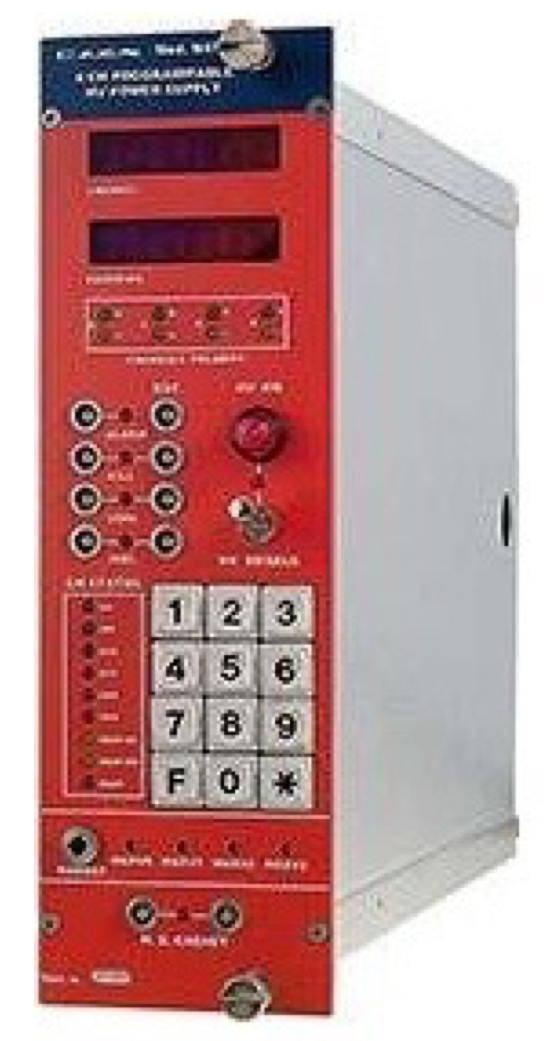
\includegraphics[height=0.25\textheight, width=\textwidth, keepaspectratio]{figures/Alim1.png}
        \caption{Alimentation de haute tension}
        \label{fig:HV1}
    \end{subfigure}
    \hfill
    \begin{subfigure}[t]{0.2\textwidth}
        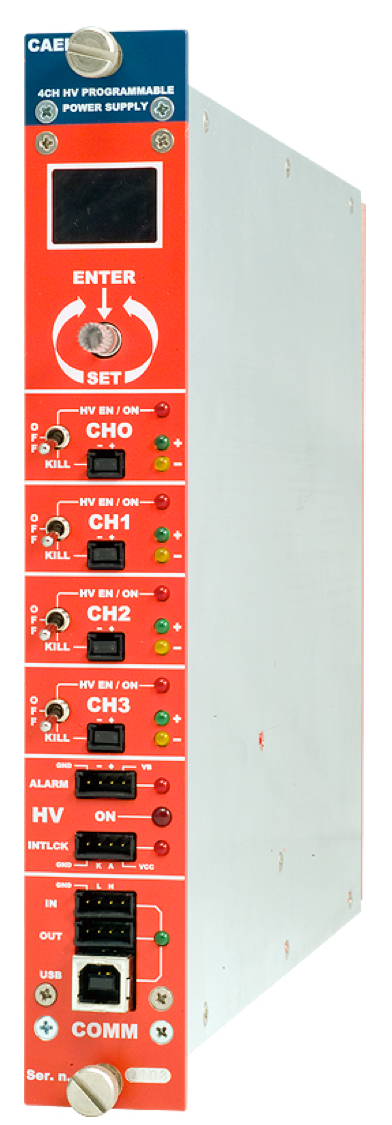
\includegraphics[height=0.25\textheight, width=\textwidth, keepaspectratio]{figures/Alim2.png}
        \caption{Alimentation de haute tension}
        \label{fig:HV2}
    \end{subfigure}
    \hfill
    \begin{subfigure}[t]{0.2\textwidth}
        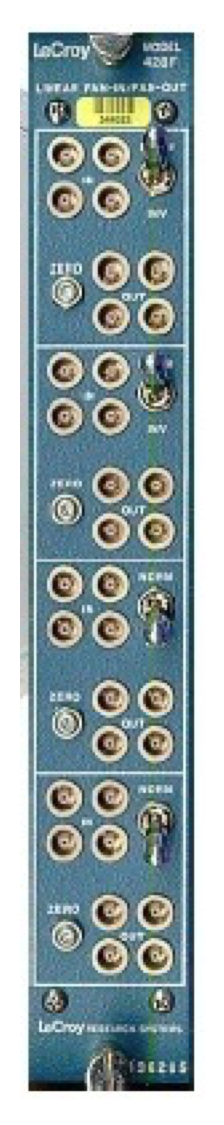
\includegraphics[height=0.25\textheight, width=\textwidth, keepaspectratio]{figures/FanInFanOut.png}
        \caption{Distributeur de signal \emph{fan-in-fan-out}}
        \label{fig:fifo}
    \end{subfigure}
    \hfill
    \begin{subfigure}[t]{0.2\textwidth}
        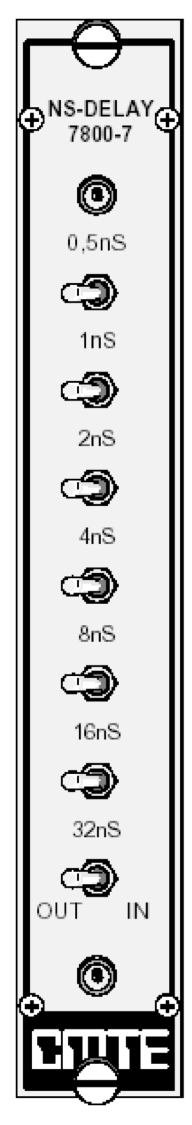
\includegraphics[height=0.25\textheight, width=\textwidth, keepaspectratio]{figures/delay.png}
        \caption{Delayeur de signal}
        \label{fig:delay}
    \end{subfigure}
    
	\vspace{1cm}
    \begin{subfigure}[t]{0.2\textwidth}
        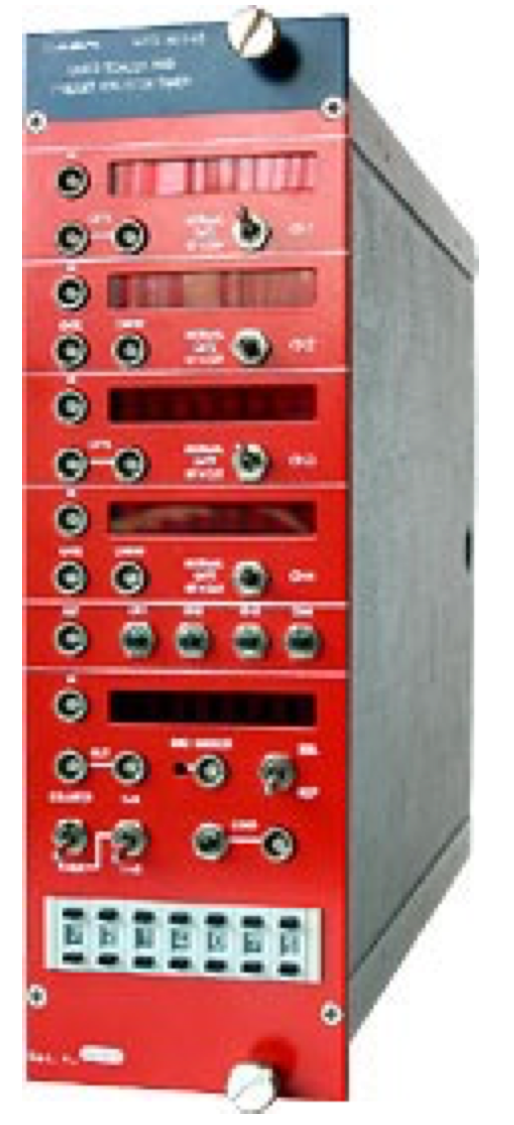
\includegraphics[height=0.25\textheight, width=\textwidth, keepaspectratio]{figures/scaler.png}
        \caption{Scaler NIM}
        \label{fig:scaler1}
    \end{subfigure}
    \hfill
    \begin{subfigure}[t]{0.25\textwidth}
        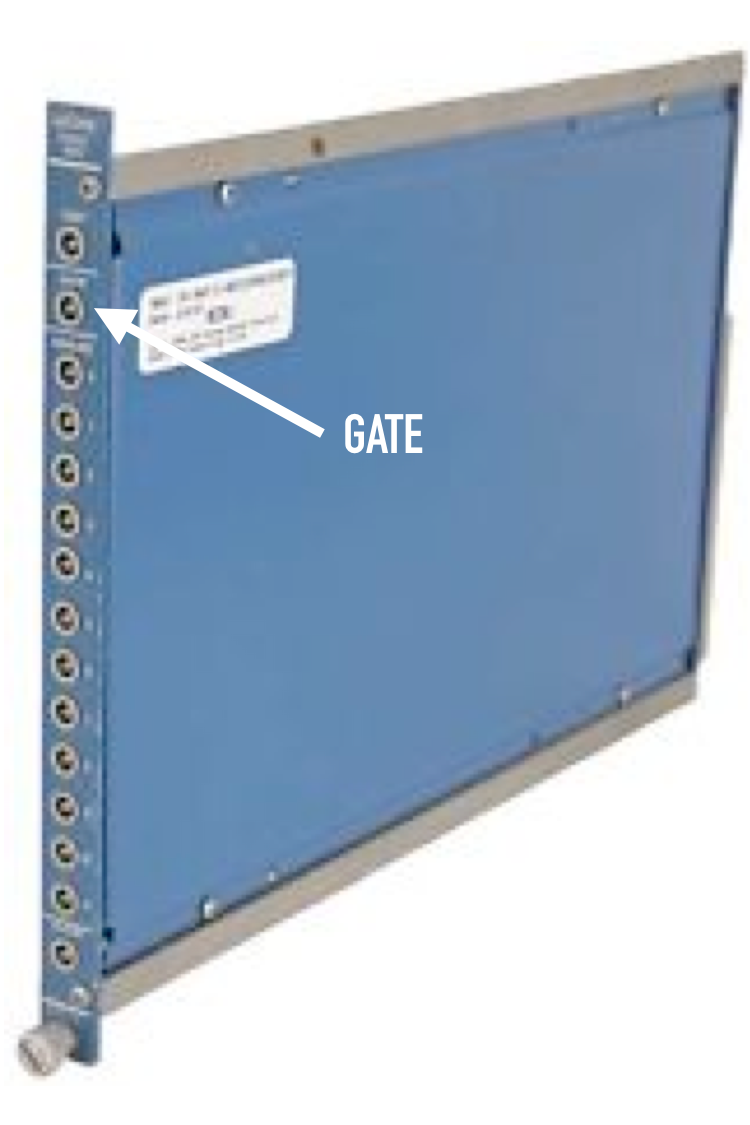
\includegraphics[height=0.25\textheight, width=\textwidth, keepaspectratio]{figures/gate.png}
        \caption{Scaler CAMAC}
        \label{fig:scaler2}
    \end{subfigure}    
    \hfill
    \begin{subfigure}[t]{0.45\textwidth}
        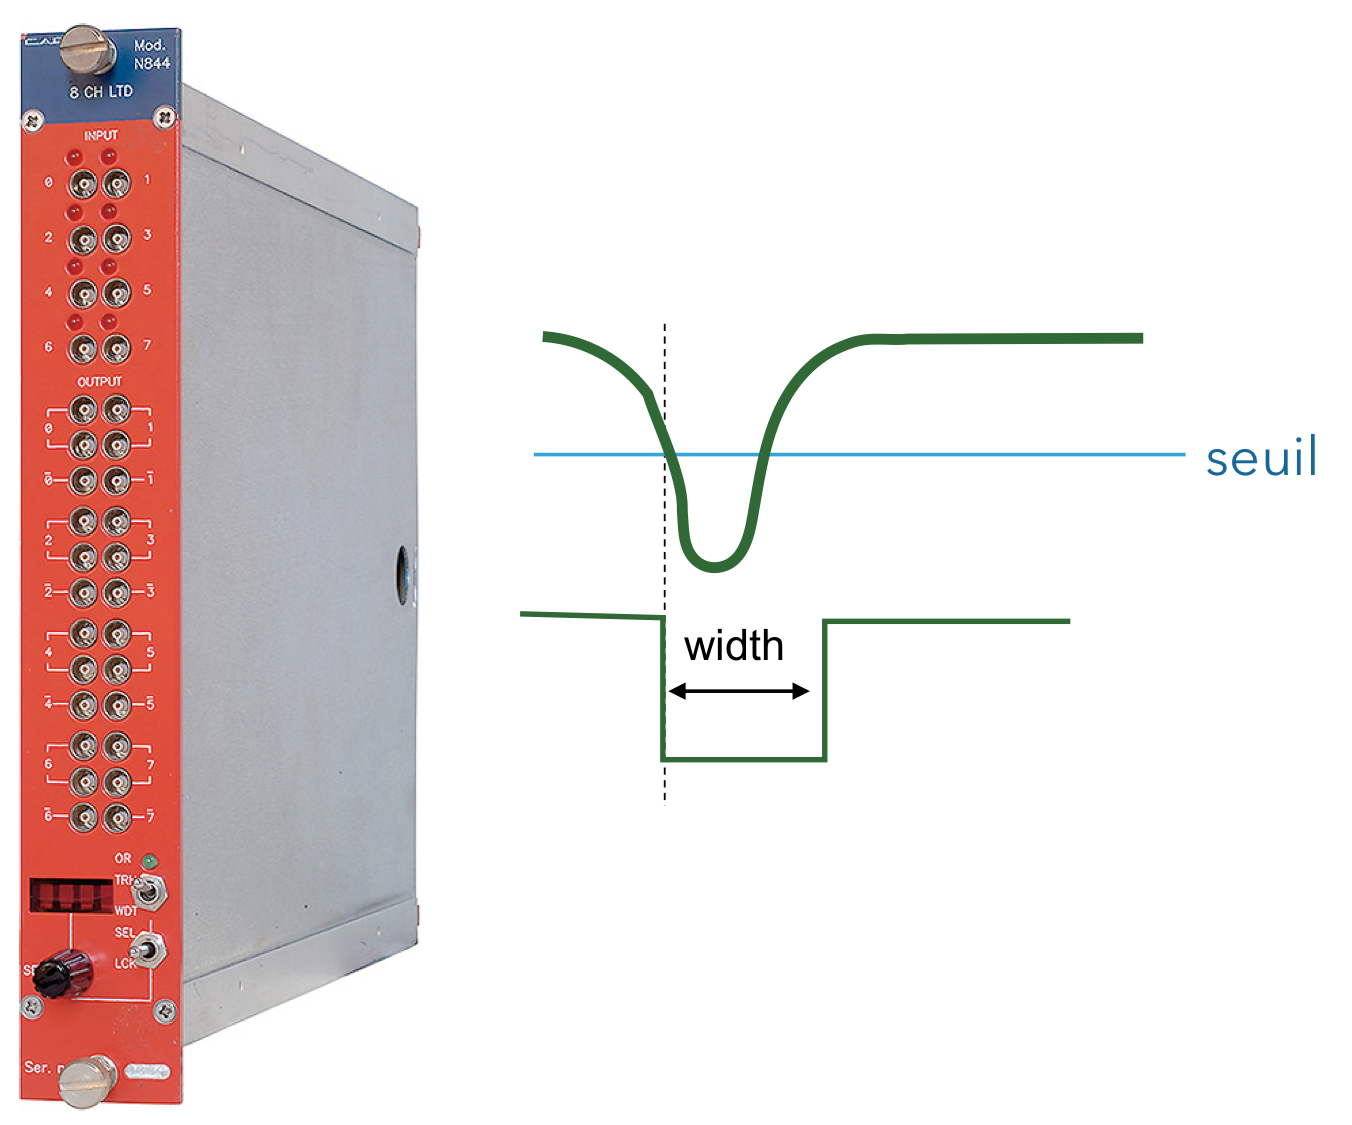
\includegraphics[height=0.3\textheight, width=\textwidth, keepaspectratio]{figures/Discriminateur.png}
        \caption{Discriminateur}
        \label{fig:discriminator}
    \end{subfigure}

	\vspace{1cm}    
    \begin{subfigure}[t]{0.45\textwidth}
        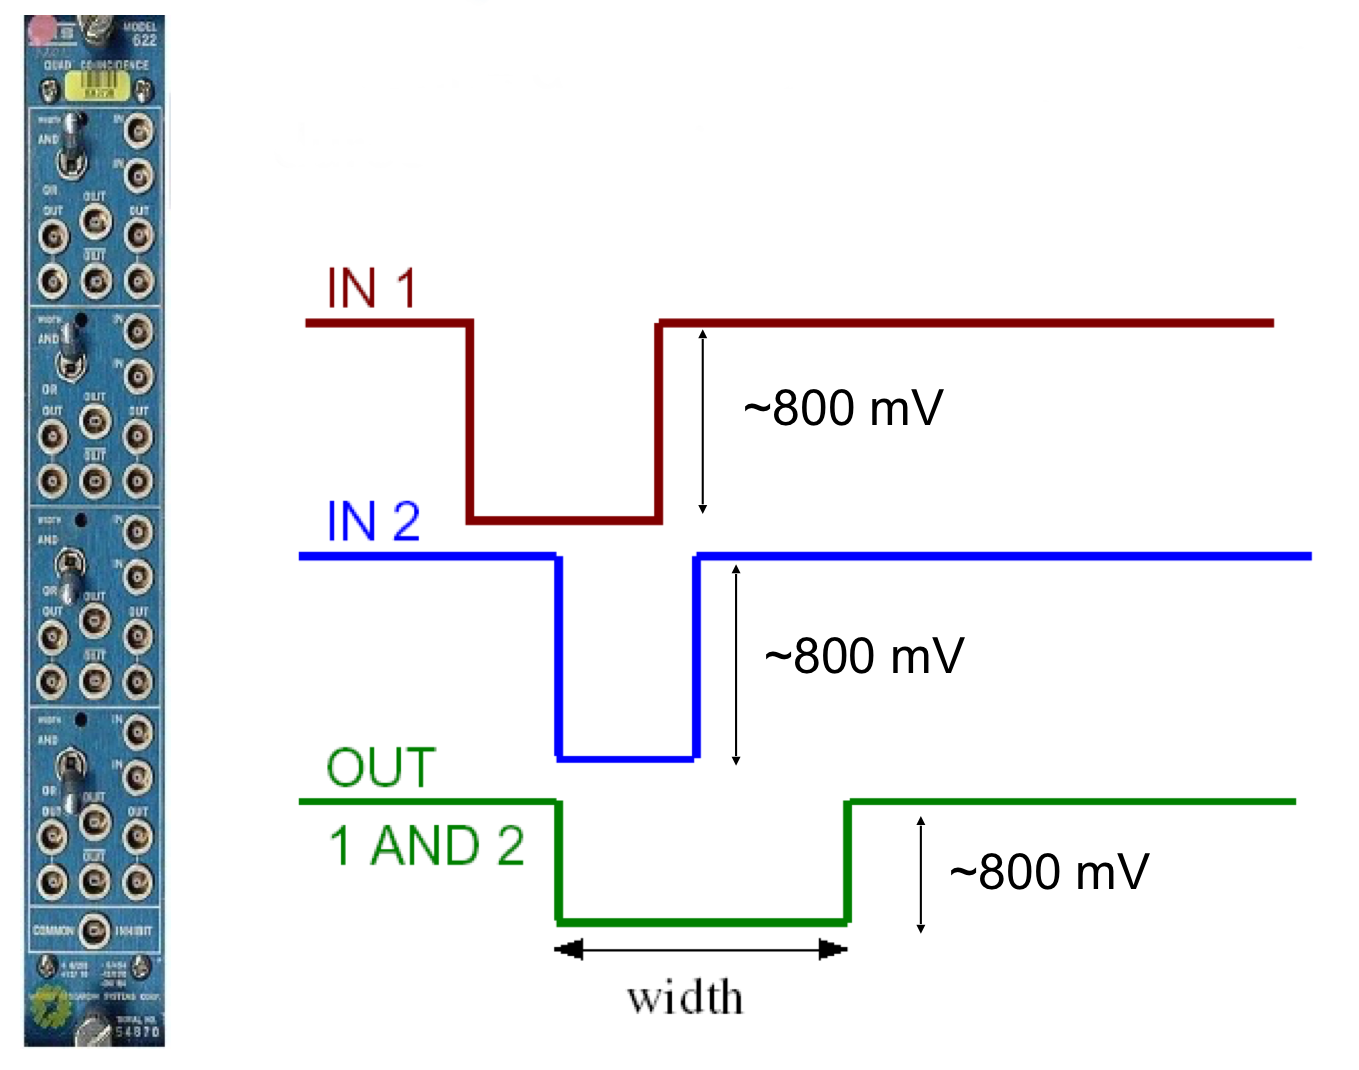
\includegraphics[height=0.3\textheight, width=\textwidth, keepaspectratio]{figures/UniteDeCoincidence_crop.png}
        \caption{Unit{\'e} de co{\"i}ncidence}
        \label{fig:coincidence}
    \end{subfigure}
    \hfill
    \begin{subfigure}[t]{0.45\textwidth}
        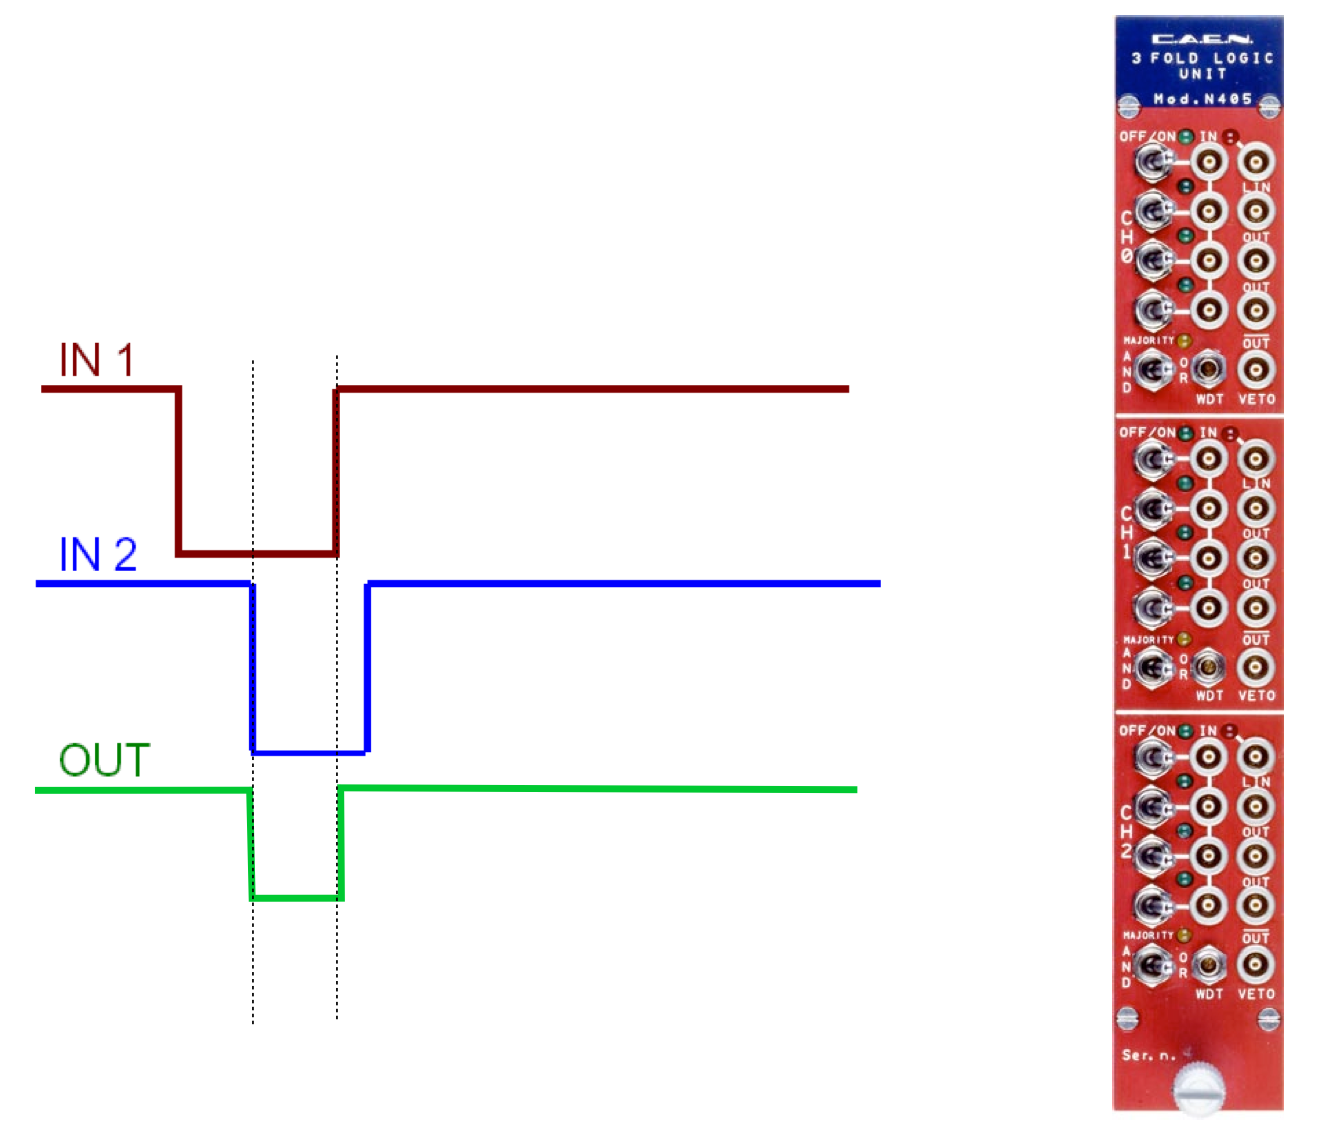
\includegraphics[height=0.3\textheight, width=\textwidth, keepaspectratio]{figures/UniteLogiqueProgrammable.png}
        \caption{Unit{\'e} logique programmable}
        \label{fig:plu}
    \end{subfigure}
    \caption{Appareils utilis{\'e}s dans les dispositifs.}
    \label{fig:devices}
\end{figure}